\section{Query Algorithms}
\label{sec:query_algorithms}

This section details the algorithms operating on the succinct DAG representation introduced in \autoref{sec:succinct_dag_representation}. The core idea is to reconstruct the necessary path weight information for a queried node $v$ by traversing the successor path starting from $v$ until an explicit node is reached, using the stored offset sequences and weights to transform the query along the way.

\subsection{Reconstructing $\mathcal{O}$-Sets}
\label{subsec:reconstructing_o_sets}

To compute queries like \Rank{}, we first need a mechanism to retrieve elements of the $\mathcal{O}$-set for any given vertex $v$. If $v$ is explicit ($v \in V_E$), this is straightforward as $\mathcal{O}_v$ is stored directly (or in a recoverable compressed format) in $\mathcal{D}[v]$. If $v$ is implicit ($v \in V_I$), the value must be reconstructed recursively by following the successor path defined by $\sigma$.

Consider the task of retrieving the $k$-th element of $\mathcal{O}_v$, denoted $\mathcal{O}_v[k]$. The stored offset sequence $\mathcal{I}_v = \mathcal{D}[v]$ provides the corresponding index $j_k = \mathcal{I}_v[k]$ in the $\mathcal{O}$-set of the successor $u = \sigma(v)$, such that $\mathcal{O}_v[k] = \mathcal{O}_u[j_k] - w(u)$. This relation forms the basis of a traversal process. We start at node $v$ with the target index $k$. We find the successor $u=\sigma(v)$ and update the target index to $j_k = \mathcal{I}_v[k]$. We also accumulate the weight $w(u)$. We repeat this process from $u$ with the new index $j_k$, following the successor path $v \to u \to \dots \to e$, where $e$ is the first explicit node encountered. Let the final index reached at node $e$ be $K$, and let the sum of weights accumulated along the path (excluding $w(v)$ but including $w(e)$ if $e \ne v$) be $W_{sum}$. The desired value $\mathcal{O}_v[k]$ is then calculated as $\mathcal{O}_e[K] - W_{sum}$.

\autoref{fig:query_path_node7} provides a concrete illustration of this query process, showing the computation of $\mathcal{O}_7[0]$ using the succinct structure from \autoref{fig:succinct_dag_example}.

\begin{figure}[htbp]
    \centering
    % \begin{tikzpicture}[
    %     node distance=1.6cm and 1.1cm, % Base distance, actual positions set via coordinates
    %     base_node/.style={circle, draw=black, thick, minimum size=9mm, inner sep=0pt, font=\sffamily},
    %     implicit_node/.style={base_node},
    %     explicit_node/.style={base_node, fill=green!40, text=black},
    %     node_label_above/.style={font=\tiny\sffamily\bfseries, text=blue!70!black, inner sep=1pt, align=center, above, yshift=1mm},
    %     node_label_below/.style={font=\tiny\sffamily\bfseries, text=blue!70!black, inner sep=1pt, align=center, below, yshift=-2mm},
    %     node_label_inside/.style={font=\tiny\sffamily\bfseries, text=blue!70!black, inner sep=0pt, align=center},
    %     step_label/.style={font=\sffamily\scriptsize, text=black, above, midway, sloped, yshift=1mm, inner sep=1pt},
    %     weight_label/.style={font=\sffamily\scriptsize, text=red!80!black, below, midway, sloped, yshift=-1mm, inner sep=1pt},
    %     annotation/.style={font=\sffamily\tiny, text=black, align=center},
    %     result_label/.style={font=\sffamily\scriptsize\bfseries, text=purple!80},
    %     successor_edge/.style={->, >={Stealth[length=2mm, width=1.5mm]}, very thick, draw=blue!65} % Pastel blue
    %     ]

    %     \node[implicit_node, label={[node_label_inside]:{$\mathcal{I}_7=(1)$}}] (N7) at (0,0) {7};
    %     \node[implicit_node, label={[node_label_above]:{$\mathcal{I}_9=(1, 2, 3)$}}] (N9) at (3,1.5) {9};
    %     \node[implicit_node, label={[node_label_below, yshift=-8mm]:{$\mathcal{I}_5=(0, 6, 7, 8)$}}] (N5) at (5.5,-0.5) {5};
    %     \node[explicit_node, label={[node_label_above]:{$\mathcal{O}_8=\{21, 23, 24, 25,$ \\ $26, 27, 29, 30, 31\}$}}] (N8) at (8.5,1.5) {8};

    %     \node[annotation, anchor=south] at ([yshift=-0.5cm]N7.south) {index $k=0$, $sum=0$};
    %     \node[annotation, anchor=north] at ([yshift=0.8cm]N9.north) {index $k=1$, $sum=9$};
    %     \node[annotation, anchor=south] at ([yshift=-0.8cm]N5.south) {index $k=2$, $sum=14$};
    %     \node[annotation, anchor=east] at ([xshift=1.6cm, yshift=-0.7cm]N8.east) {index $k=7$, $sum=22$};

    %     \draw [successor_edge] (N7) -- node[step_label] {Use $\mathcal{I}_7[0]=\mathbf{1}$}
    %     node[weight_label] {$+ w(9)=9$} (N9);
    %     \draw [successor_edge] (N9) -- node[step_label] {Use $\mathcal{I}_9[1]=\mathbf{2}$}
    %     node[weight_label] {$+ w(5)=5$} (N5);
    %     \draw [successor_edge] (N5) -- node[step_label] {Use $\mathcal{I}_5[2]=\mathbf{7}$}
    %     node[weight_label] {$+ w(8)=8$} (N8);

    %     \node[annotation, below=1.1cm of N8, xshift=0.4cm] (Calc) {Retrieve $\mathcal{O}_8[7] = 30$. \\ Final Result = $30 - sum = 30 - 22 = \mathbf{8}$.};
    %     \node[result_label, below=0.1cm of Calc] {Result: $\mathcal{O}_7[0] = 8$};

    % \end{tikzpicture}
    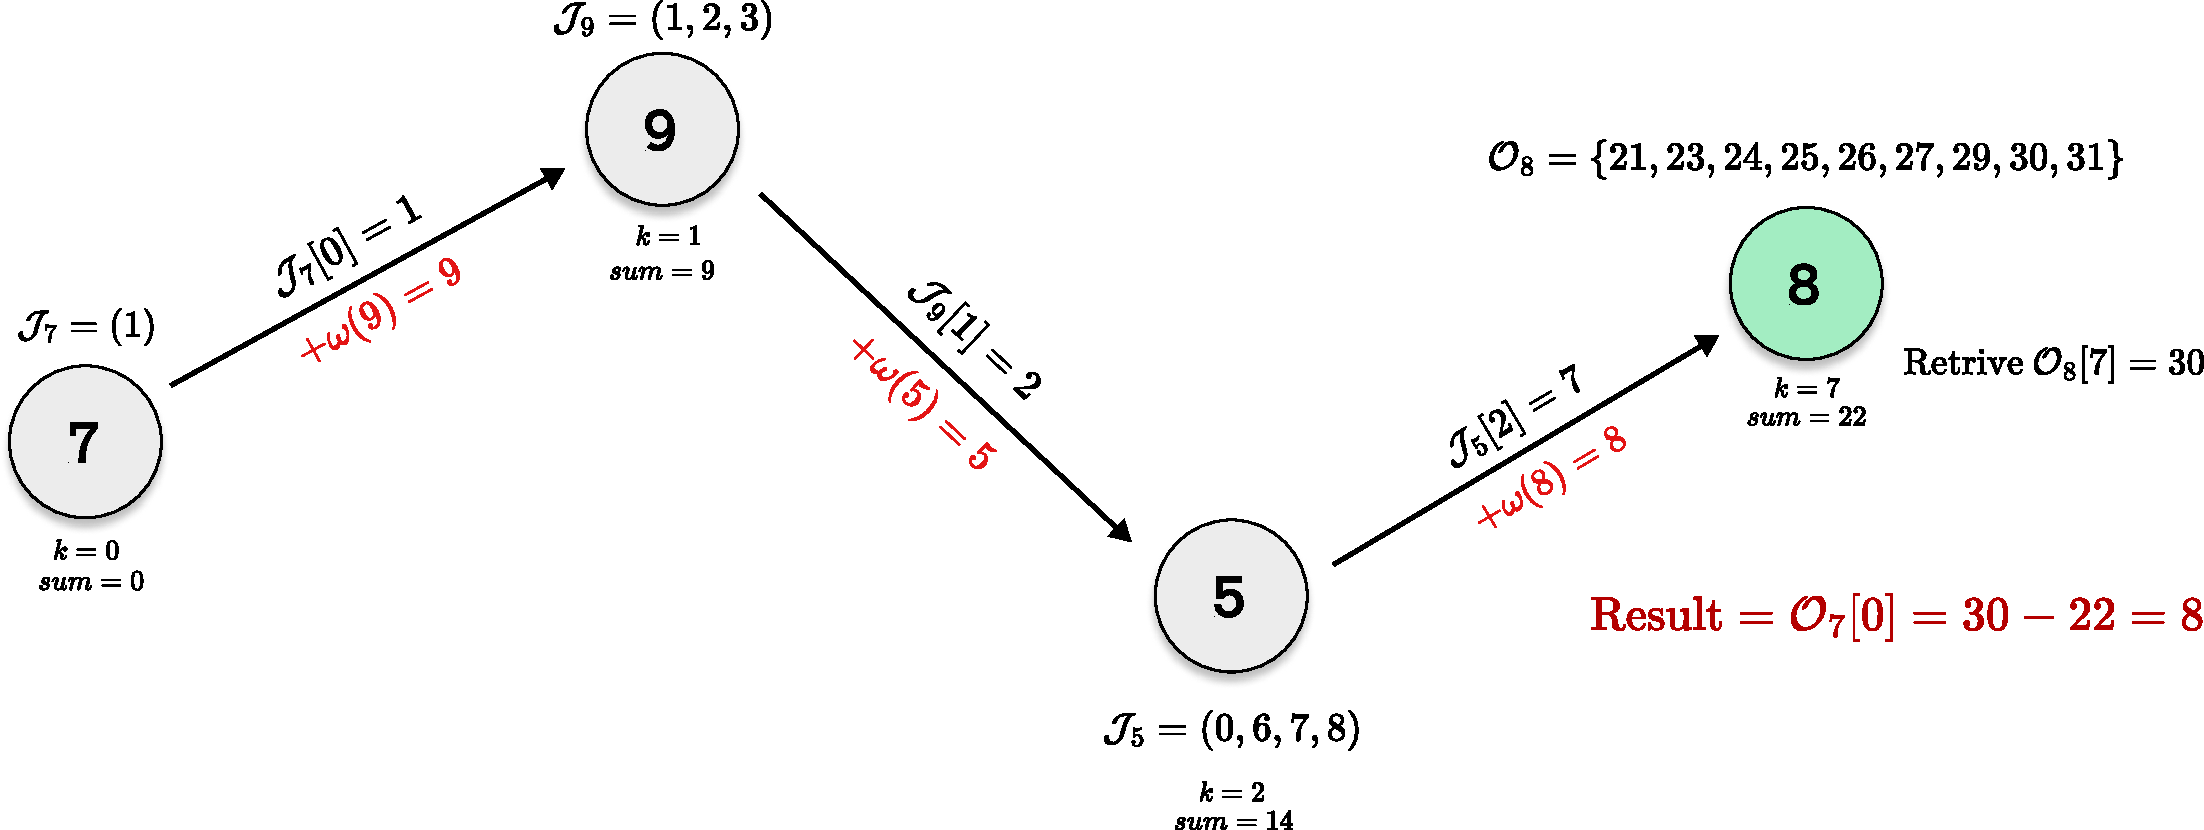
\includegraphics[width=\textwidth]{assets/dag_query4.pdf}
    \caption{Visualization of the query process for retrieving the element at index $k=0$ of $\mathcal{O}_7$ using the succinct representation (\autoref{fig:succinct_dag_example}). The query follows the successor path $7 \to 9 \to 5 \to 8$. At each step from an implicit node $v$ to its successor $u=\sigma(v)$, the current index $k_{current}$ is updated using the stored offset $k_{next} = \mathcal{I}_v[k_{current}]$, and the weight $w(u)$ is added to an accumulator (sum). The path starts with $k=0$ at node 7. It proceeds to node 9 using index $\mathcal{I}_7[0]=1$, accumulating $w(9)=9$. Then to node 5 using index $\mathcal{I}_9[1]=2$, accumulating $w(5)=5$ (total sum 14). Then to node 8 using index $\mathcal{I}_5[2]=7$, accumulating $w(8)=8$ (total sum 22). Node 8 is explicit, so the value at the final index 7, $\mathcal{O}_8[7]=30$, is retrieved. The result is obtained by subtracting the total accumulated weight: $30 - 22 = 8$. This correctly reconstructs $\mathcal{O}_7[0]$.}
    \label{fig:query_path_node7}
\end{figure}

The general procedure to compute the $k$-th element ($0$-indexed) of $\mathcal{O}_v$ is formalized in Algorithm \ref{alg:get_value}. It implements the traversal and accumulation process described above, relying on accessing the structure components: weights $\mathcal{W}$, successor information $\Sigma$ (to get $\sigma(v)$ and check for explicit nodes), and associated data $\mathcal{D}$ (to retrieve $\mathcal{I}$ sequences or $\mathcal{O}$-sets)

\begin{algorithm}
    \caption{$\textsc{GetValue}(v, k)$: Compute the $k$-th element of $\mathcal{O}_v$}
    \label{alg:get_value}
    \small
    \begin{algorithmic}[1]
        \Require Vertex ID $v$, index $k \in \{0, \dots, |\mathcal{O}_v|-1\}$.
        \Ensure The value of the $k$-th smallest element in $\mathcal{O}_v$.
        \State $current\_node \gets v$
        \State $current\_index \gets k$
        \State $weight\_sum \gets 0$
        \While{$current\_node \notin V_E$}
        \State $successor \gets \Sigma[current\_node]$
        \State $weight\_sum \gets weight\_sum + \mathcal{W}[successor]$
        \State $\mathcal{I}_{current\_node} \gets \mathcal{D}[current\_node]$
        \State $next\_index \gets \mathcal{I}_{current\_node}[current\_index]$
        \State $current\_node \gets successor$
        \State $current\_index \gets next\_index$
        \EndWhile

        \State $\mathcal{O}_{explicit} \gets \mathcal{D}[current\_node)$
        \State $base\_value \gets \mathcal{O}_{explicit}[current\_index]$
        \State \Return $base\_value - weight\_sum$
    \end{algorithmic}
\end{algorithm}

The correctness of Algorithm \ref{alg:get_value} follows inductively from the definition of the offset sequence $\mathcal{I}_v$. Let $x_k^{(v)}$ denote the $k$-th element of $\mathcal{O}_v$. If $v$ is implicit with successor $u = \sigma(v)$, then by construction $x_k^{(v)} = x_{j_k}^{(u)} - w(u)$, where $j_k = \mathcal{I}_v[k]$. The algorithm iteratively applies this relation: if $v \to u \to \dots \to e$ is the successor path ending at an explicit node $e$, and the indices transform as
\[ k \to j_k^{(v)} \to j_{j_k^{(v)}}^{(u)} \to \dots \to K \]
then the algorithm computes
\[x_K^{(e)} - \sum_{z \in \text{path } v \to e, z \neq v} w(z)\]
which correctly yields $x_k^{(v)}$.

To reconstruct the entire $\mathcal{O}$-set for a vertex $v$, we can repeatedly call $\textsc{GetValue}(v, k)$ for $k=0, 1, \dots, |\mathcal{O}_v|-1$. This requires knowing the size $|\mathcal{O}_v|$. We assume this size information is either stored explicitly for each node or can be efficiently derived (e.g., potentially stored alongside $\mathcal{I}_v$ or $\mathcal{O}_v$ in the $\mathcal{D}$ component). Let $\textsc{Length}(v)$ be an operation that returns $|\mathcal{O}_v|$. This procedure is implemented in Algorithm \ref{alg:get_o_set}.

\begin{algorithm}
    \caption{$\textsc{GetOSet}(v)$: Reconstruct the $\mathcal{O}$-set for vertex $v$}
    \label{alg:get_o_set}
    \small
    \begin{algorithmic}[1]
        \Require Vertex ID $v$.
        \Ensure The sorted sequence $\mathcal{O}_v$.
        \State $size \gets \textsc{Length}(v)$
        \State Initialize an empty list $O\_list$ of size $size$.
        \For{$k$ from $0$ to $size - 1$}
        \State $value \gets \textsc{GetValue}(v, k)$
        \State $O\_list[k] \gets value$
        \EndFor
        \State \Return $O\_list$
    \end{algorithmic}
\end{algorithm}

\subsection{Computing the Rank Query}
\label{subsec:computing_rank}

Equipped with the ability to reconstruct $\mathcal{O}_N$ for any query vertex $N$ via Algorithm \ref{alg:get_o_set}, we can now implement the \Rank{} query as specified in \ref{def:rank_dag}. The procedure involves two main steps: first, generate the initial set of intervals based on the elements of $\mathcal{O}_N$ and the weight $w(N)$; second, merge these potentially overlapping or adjacent intervals into a minimal set of disjoint intervals.

The interval merging step is a standard procedure. Given a list of intervals sorted by their starting points, we can merge them efficiently. The core idea is to iterate through the sorted intervals, merging the current interval with the next one if they overlap or are directly adjacent (i.e., the start of the next interval is less than or equal to the end of the current interval plus one). Algorithm \ref{alg:merge_intervals} formalizes this merging process, which requires linear time with respect to the number of initial intervals
\begin{algorithm}[htbp]
    \caption{$\textsc{MergeIntervals}(Intervals)$: Merge sorted intervals}
    \label{alg:merge_intervals}
    \small
    \begin{algorithmic}[1]
        \Require A list $Intervals = \{[l_1, r_1], [l_2, r_2], \dots\}$ sorted by start points $l_i$.
        \Ensure A minimal list $MergedIntervals$ of disjoint intervals
        \State Initialize an empty list $MergedIntervals$.
        \If{$Intervals$ is not empty}
        \State $current\_interval \gets Intervals[0]$.
        \For{$i$ from $1$ to length$(Intervals) - 1$}
        \State $next\_interval \gets Intervals[i]$.
        \If{$next\_interval.l \le current\_interval.r + 1$}
        \State $current\_interval.r \gets \max(current\_interval.r, next\_interval.r)$
        \Else
        \State Append $current\_interval$ to $MergedIntervals$.
        \State $current\_interval \gets next\_interval$.
        \EndIf
        \EndFor
        \State Append $current\_interval$ to $MergedIntervals$.
        \EndIf
        \State \Return $MergedIntervals$.
    \end{algorithmic}
\end{algorithm}


% Algorithm \ref{alg:rank_dag} implements the Rank query defined in \ref{def:rank_dag}. It first reconstructs the necessary path weight information ($\mathcal{O}_N$), then applies the specified transformation to generate the initial set of intervals
% \[S_N = \bigcup_{x \in \mathcal{O}_N} [ \max(0, x - w_N + 1), x ]\]
% Finally, it employs the standard interval merging algorithm to produce the canonical representation $\mathcal{R}_N$ as a minimal set of disjoint intervals. Note that the sorting step (line 9) is necessary because intervals generated from consecutive elements in $\mathcal{O}_N$ are not guaranteed to have non-decreasing start points.

Algorithm \ref{alg:rank_dag} implements the Rank query defined in \ref{def:rank_dag}. It begins by reconstructing the set $\mathcal{O}_N$ using $\textsc{GetOSet}$ (Algorithm \ref{alg:get_o_set}). Then, for each path weight $x \in \mathcal{O}_N$, it generates the interval $[\max(0, x - w_N + 1), x]$ according to the transformation rule specified in Definition \ref{def:rank_dag}, where $w_N = \mathcal{W}[N]$. The union of these generated intervals constitutes the set $S_N$:
\[ S_N = \bigcup_{x \in \mathcal{O}_N} [ \max(0, x - w_N + 1), x ]. \]
Since these intervals may overlap or be adjacent, they are first sorted by their starting points. The sorted intervals are then merged via Algorithm \ref{alg:merge_intervals} (line 10) to compute the final result $\mathcal{R}_N$, which is the minimal representation of $S_N$ as disjoint intervals.

\begin{algorithm}
    \caption{$\mathrm{Rank}_G(N)$: Compute the Rank query for vertex $N$}
    \label{alg:rank_dag}
    \small
    \begin{algorithmic}[1]
        \Require Vertex ID $N$.
        \Ensure A minimal set of disjoint intervals $\mathcal{R}_N$ representing $S_N$
        \State $\mathcal{O}_N \gets \textsc{GetOSet}(N)$
        \State $w_N \gets \mathcal{W}[N]$
        \State Initialize an empty list $InitialIntervals$.
        \For{each $x \in \mathcal{O}_N$}
        \State $l \gets \max(0, x - w_N + 1)$
        \State $r \gets x$
        \State Append the interval $[l, r]$ to $InitialIntervals$.
        \EndFor
        \State Sort $InitialIntervals$ based on the starting point $l$.
        \State $MergedIntervals \gets \textsc{MergeIntervals}(InitialIntervals)$
        \State \Return $MergedIntervals$.
    \end{algorithmic}
\end{algorithm}


\subsubsection*{Example: Rank Query Computation}
\label{subsubsec:rank_query_example_node2}

We illustrate the execution of Algorithm \ref{alg:rank_dag} to compute $\mathrm{Rank}_G(N)$ for vertex $N=2$. Referring to the example structure presented in \autoref{fig:dag_example} and \autoref{fig:succinct_dag_example}, this vertex has weight $w(2)=2$.

First, the computation requires the $\mathcal{O}$-set for node 2. The algorithm calls $\textsc{GetOSet}(2)$ (Algorithm \ref{alg:get_o_set}), which utilizes $\textsc{GetValue}(2, k)$ (Algorithm \ref{alg:get_value}) for $k=0, 1, \dots, |\mathcal{O}_2|-1$. As described previously (Section \ref{subsec:reconstructing_o_sets} and Figure \ref{fig:query_path_node7} show a similar process), $\textsc{GetValue}$ traverses the successor path determined by $\sigma$. For node 2, this path is $2 \to 10 \to 8$. By following this path, applying the offset indices $\mathcal{I}_2 = \mathcal{D}[2]$ and $\mathcal{I}_{10} = \mathcal{D}[10]$, accumulating the weights $w(10) = \mathcal{W}[10]$ and $w(8) = \mathcal{W}[8]$, and retrieving the base value from the explicit node's data $\mathcal{D}[8]=\mathcal{O}_8$, the set $\mathcal{O}_2 = \{5, 9, 11\}$ is reconstructed.

Next, the weight of the query node, $w_N = w(2) = 2$, is retrieved (from $\mathcal{W}[2]$).

The algorithm then proceeds to generate the initial set of intervals. Each element $x \in \mathcal{O}_2$ is transformed into an interval $[\max(0, x - w_2 + 1), x]$ using the rule from Definition \ref{def:rank_dag}:
\begin{align*}
    x=5 \quad  & \longrightarrow \quad [\max(0, 5 - 2 + 1), 5] = [4, 5]     \\
    x=9 \quad  & \longrightarrow \quad [\max(0, 9 - 2 + 1), 9] = [8, 9]     \\
    x=11 \quad & \longrightarrow \quad [\max(0, 11 - 2 + 1), 11] = [10, 11]
\end{align*}
This yields the initial list of intervals
\[InitialIntervals = \{ [4, 5], [8, 9], [10, 11] \}.\]
Finally, $\textsc{MergeIntervals}$ (Algorithm \ref{alg:merge_intervals}) is applied to this list\footnote{after sorting, which does not change the order in this specific case.}. The intervals $[8, 9]$ and $[10, 11]$ merge because $10 \le 9+1$, resulting in $[8, 11]$. The interval $[4, 5]$ remains distinct as $8 > 5+1$. The final result returned by $\mathrm{Rank}_G(2)$ is the minimal set of disjoint intervals $\mathcal{R}_2 = \{ [4, 5], [8, 11] \}$.
